\subsection{Response to lighting changes}
\label{sec:lighting}

\begin{figure*}[t]
  \centering
  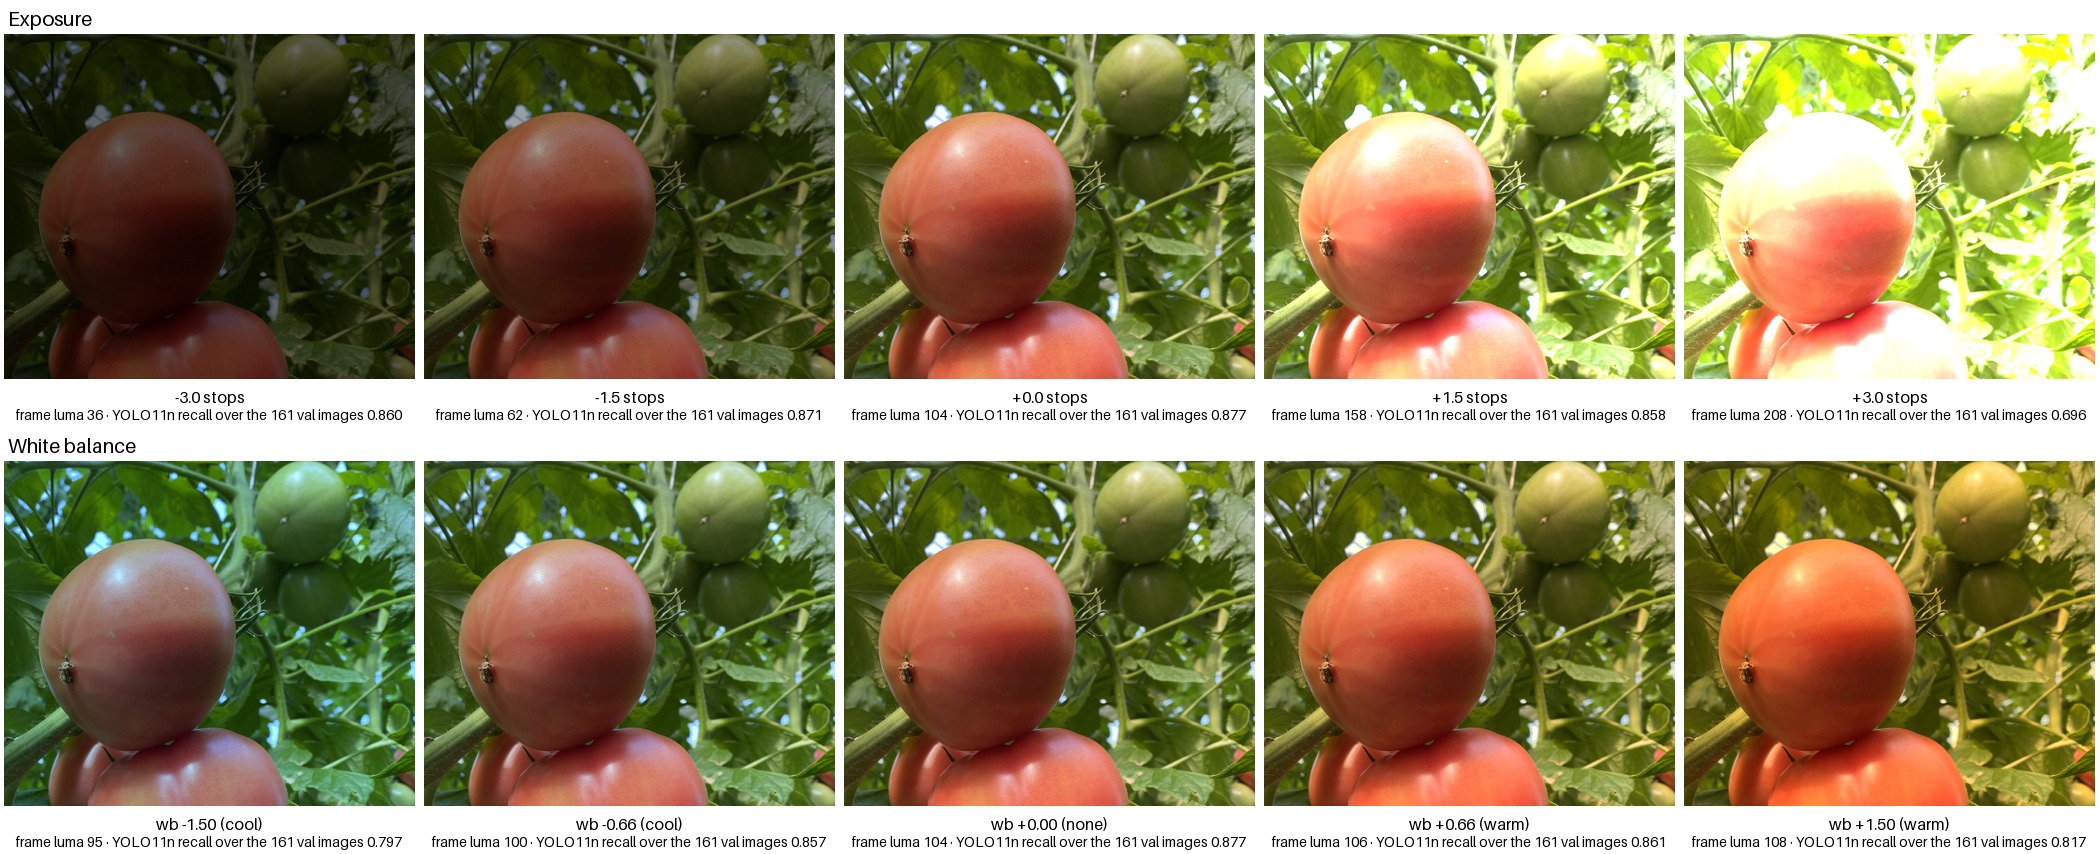
\includegraphics[width=\textwidth]{lighting_examples.jpg}
  \caption{One validation frame under the photometric interventions: exposure
  from $-3$ to $+3$ stops (top) and white balance from cool to warm (bottom).
  Captions give the mean luma of the frame and the baseline detector's recall
  over the whole validation split at that level. Annotations are never moved;
  only the pixels change.}
  \label{fig:lighting-examples}
\end{figure*}

\begin{table}[t]
\caption{Recall at confidence 0.25 and counting MAE at the best threshold under
the four extreme lighting conditions. One seed per row; the colour-augmentation
rows are repeated over three seeds in Table~\ref{tab:seeds}.}
\label{tab:lighting}
\centering
\begin{tabular}{lrrrrr}
\toprule
Model & clean & $-3$ st. & $+3$ st. & cool & warm \\
\midrule
YOLO11n & 0.877 & 0.860 & 0.696 & 0.797 & 0.817 \\
\quad no colour jitter & 0.877 & 0.765 & 0.608 & 0.751 & 0.782 \\
\quad hsv\_v08 & 0.874 & 0.870 & 0.692 & 0.810 & 0.820 \\
\quad hsv\_wide & 0.871 & 0.868 & 0.704 & 0.824 & 0.847 \\
YOLO11s & 0.916 & 0.904 & 0.739 & 0.842 & 0.883 \\
YOLO11m & 0.935 & 0.901 & 0.786 & 0.870 & 0.898 \\
YOLO11l & 0.929 & 0.912 & 0.782 & 0.877 & 0.901 \\
YOLO11x & 0.935 & 0.914 & 0.730 & 0.865 & 0.899 \\
\midrule
\multicolumn{6}{l}{\emph{counting MAE at the best threshold}} \\
YOLO11n & 0.96 & 1.13 & 1.78 & 1.31 & 1.35 \\
\quad no colour jitter & 1.00 & 1.47 & 2.07 & 1.52 & 1.71 \\
YOLO11m & 0.88 & 1.05 & 1.68 & 1.11 & 1.27 \\
YOLO11x & 0.87 & 0.93 & 1.81 & 1.23 & 1.06 \\
\bottomrule
\end{tabular}
\end{table}

Table~\ref{tab:lighting} compares model size and lighting changes using the same
recall scale. Moving from YOLO11n to YOLO11x raises recall on clean frames by
0.058. Over-exposing the same frames by three stops reduces recall for the best
model in the ladder by 0.205.

The response differs between the two exposure directions. At $-3$ stops (mean
luma 42 out of 255), recall falls by at most 0.03 for any model. It does not
fall for the variants with the widest jitter. At $+3$ stops, recall drops by
0.15 to 0.21 and counting MAE roughly doubles. The examples in
Figure~\ref{fig:lighting-examples} indicate a possible explanation. Darkening
compresses the signal while preserving the ratios between channels. Clipping
removes those ratios, and an over-exposed red tomato loses the saturation used
to assign its stage. Additional capacity does not recover this information.
YOLO11x performs no better at $+3$ stops than YOLO11s.

The two white-balance directions also produce different results. A cool cast
reduces recall more than a warm cast of the same magnitude. A warm cast has a
larger effect on counting than on detection. It moves green and half-ripened
fruit along the green-to-red axis towards riper predictions, causing the ripe
stage to be over-counted. The annotation disagreement measured in
Section~\ref{sec:colour} also shifts the apparent colour boundary along this
axis. The camera causes the shift in the lighting test, while the annotators
cause it in the cross-dataset test.

\begin{figure}[t]
  \centering
  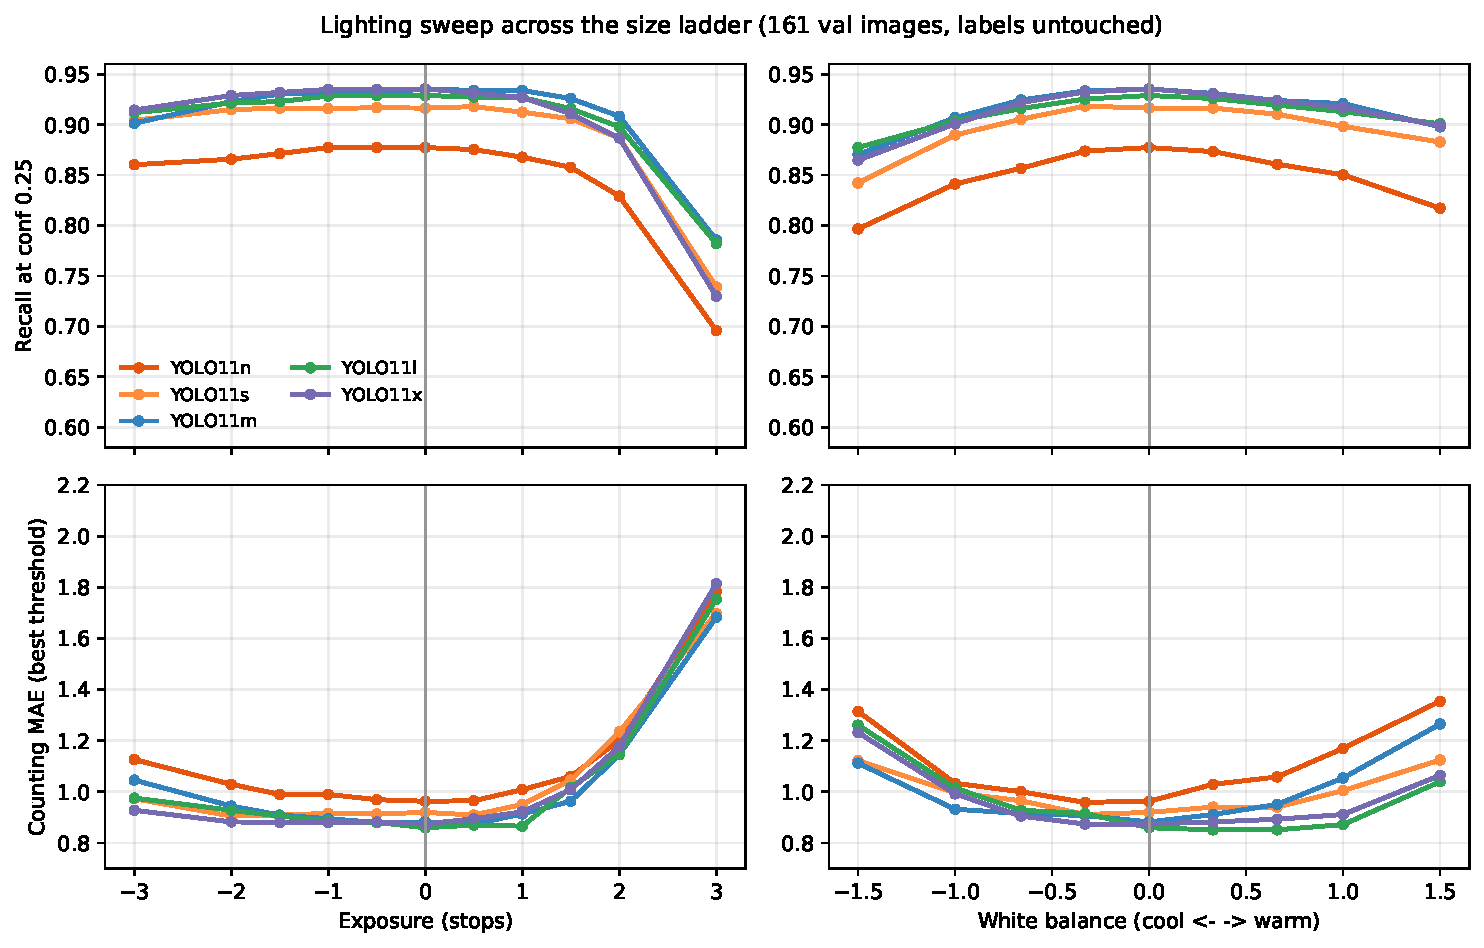
\includegraphics[width=\columnwidth]{lighting_sizes.pdf}
  \caption{Recall at a fixed threshold and counting error at the best threshold
  along the exposure and white-balance axes for the whole size ladder. The
  curves are ordered by capacity on clean frames and converge at the extremes.}
  \label{fig:lighting-sizes}
\end{figure}

\subsection{Effect of wider colour augmentation}
\label{sec:hsv}

\begin{figure}[t]
  \centering
  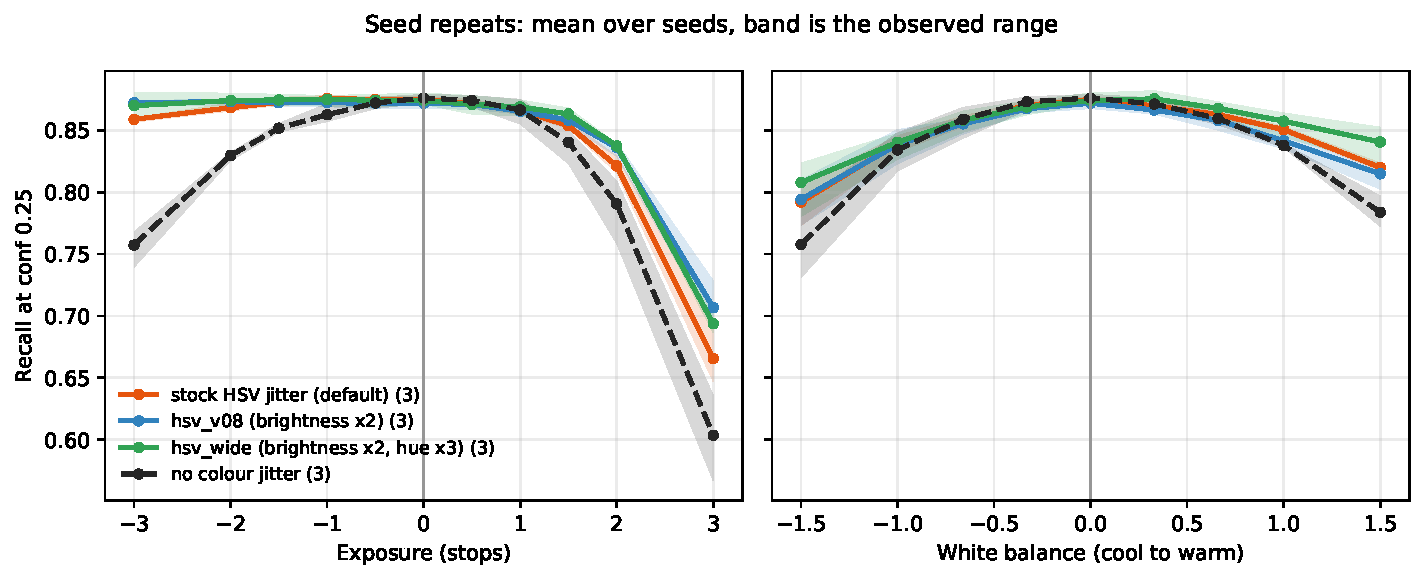
\includegraphics[width=\columnwidth]{lighting_seeds.pdf}
  \caption{Three seeds per training recipe. The line is the mean over seeds and
  the band is the observed range. Removing colour jitter separates from the
  three jittered recipes only once the frame is perturbed, and the seed spread
  itself widens with the perturbation.}
  \label{fig:lighting-seeds}
\end{figure}

\begin{table}[t]
\caption{Colour-augmentation recipes over three seeds: recall at confidence
0.25, mean (observed range). The spread of the default recipe against itself is
the noise floor for this comparison.}
\label{tab:seeds}
\centering
\begin{tabular}{lrrrr}
\toprule
Recipe & clean & $-3$ st. & $+3$ st. & cool \\
\midrule
default & 0.875 & 0.859 & 0.666 & 0.792 \\
 & \scriptsize(0.874--0.877) & \scriptsize(0.857--0.860) & \scriptsize(0.647--0.696) & \scriptsize(0.773--0.807) \\
\texttt{hsv\_v08} & 0.872 & \textbf{0.872} & \textbf{0.707} & 0.794 \\
 & \scriptsize(0.868--0.875) & \scriptsize(0.870--0.874) & \scriptsize(0.692--0.728) & \scriptsize(0.774--0.810) \\
\texttt{hsv\_wide} & 0.874 & 0.870 & 0.694 & \textbf{0.808} \\
 & \scriptsize(0.871--0.880) & \scriptsize(0.862--0.881) & \scriptsize(0.686--0.704) & \scriptsize(0.781--0.824) \\
\texttt{no\_colour} & 0.876 & 0.757 & 0.604 & 0.758 \\
 & \scriptsize(0.872--0.879) & \scriptsize(0.739--0.768) & \scriptsize(0.567--0.636) & \scriptsize(0.731--0.791) \\
\bottomrule
\end{tabular}
\end{table}

\begin{table}[t]
\caption{Each recipe against the default, seed-averaged and paired over the 161
validation images. $\Delta$MAE is the change in counting error, negative
favouring the recipe; $\Delta$recall is at confidence 0.25. Brackets are 95\%
bootstrap intervals and $p$ is Holm-adjusted over the five levels.}
\label{tab:seed-tests}
\centering
\begin{tabular}{llrr}
\toprule
Recipe & Level & $\Delta$MAE [95\% CI] & $\Delta$recall \\
\midrule
\texttt{hsv\_v08}  & clean    & $+0.005$ [$-0.039$, $+0.049$] & $-0.003$ \\
                   & $-3$ st. & $-0.075$ [$-0.130$, $-0.022$]$^{*}$ & $+0.013$ \\
                   & $+3$ st. & $-0.136$ [$-0.260$, $-0.039$]$^{*}$ & $+0.041$ \\
                   & cool     & $-0.062$ [$-0.133$, $+0.008$] & $+0.002$ \\
                   & warm     & $+0.039$ [$-0.021$, $+0.101$] & $-0.005$ \\
\midrule
\texttt{hsv\_wide} & clean    & $+0.062$ [$+0.007$, $+0.116$] & $-0.001$ \\
                   & $-3$ st. & $-0.035$ [$-0.101$, $+0.029$] & $+0.011$ \\
                   & $+3$ st. & $-0.045$ [$-0.138$, $+0.039$] & $+0.028$ \\
                   & cool     & $-0.168$ [$-0.261$, $-0.075$]$^{**}$ & $+0.016$ \\
                   & warm     & $-0.001$ [$-0.108$, $+0.093$] & $+0.021$ \\
\midrule
\texttt{no\_colour}& clean    & $-0.043$ [$-0.103$, $+0.017$] & $+0.001$ \\
                   & $-3$ st. & $+0.324$ [$+0.208$, $+0.450$]$^{***}$ & $-0.102$ \\
                   & $+3$ st. & $+0.165$ [$+0.058$, $+0.280$]$^{**}$ & $-0.062$ \\
                   & cool     & $+0.203$ [$+0.115$, $+0.295$]$^{***}$ & $-0.034$ \\
                   & warm     & $+0.226$ [$+0.100$, $+0.364$]$^{**}$ & $-0.036$ \\
\bottomrule
\multicolumn{4}{l}{\scriptsize $^{*}p<0.05$, $^{**}p<0.01$, $^{***}p<0.001$, Holm-adjusted} \\
\end{tabular}
\end{table}

This section tests whether stronger photometric augmentation improves robustness
to the lighting interventions. We first measure variation across seeds because
it is similar in magnitude to the effects being compared.

The spread across seeds depends on the lighting level. Retraining the
\emph{same} default recipe at three seeds changes clean recall by 0.003. At
$+3$ stops, recall changes by 0.049, from 0.647 to 0.696
(Table~\ref{tab:seeds}). The single-seed value of 0.696 for the default at $+3$
stops in Table~\ref{tab:lighting} is the most favourable of its three runs. A
conclusion based on one run at this extreme level would therefore be within the
observed retraining variation.

\textbf{Removing colour jitter has no detectable effect on clean frames but a
large effect under perturbation.} On clean frames, \texttt{no\_colour} is
indistinguishable from the default. Its recall is $+0.001$, and its counting
error is $0.043$ \emph{lower} with an interval that spans zero ($p=0.16$).
Under every perturbation, it gives lower recall: $-0.102$ at $-3$ stops,
$-0.062$ at $+3$, and $-0.034$ and $-0.036$ under the two colour casts. Its
counting error is also worse by 0.17 to 0.32, with Holm-adjusted $p \le 0.006$
at each of the four levels (Table~\ref{tab:seed-tests}). An ablation evaluated
only on clean held-out frames would therefore recommend removing an
augmentation that improves every perturbed condition tested here.

\textbf{Widening the jitter produces smaller, perturbation-specific gains.}
Doubling the brightness half-width improves the two exposure extremes. At $+3$
stops, the changes are $-0.136$ counting error and $+0.041$ recall. At $-3$
stops, they are $-0.075$ and $+0.013$. Both results are significant after
correction, while neither white-balance level differs from the default.
Widening hue produces its clearest changes under the white-balance intervention.
At a cool cast, the changes are $-0.168$ counting error ($p=0.002$) and $+0.016$
recall. Recall changes by $+0.021$ at a warm cast. Its exposure changes remain
within the interval, and clean-frame counting error increases by $+0.062$; this
increase is not significant after correction.

Each modified component improves the corresponding type of perturbation.
Increasing the brightness half-width improves the two exposure conditions.
Widening hue, the HSV change most similar to a colour cast, improves the two
white-balance conditions. Neither modification produces an improvement across
all photometric conditions.

The effect sizes support retaining the default recipe. Removing the jitter
reduces recall by up to 0.102. Widening it improves recall by at most 0.041 and
only for the corresponding perturbation. If a deployment is known to encounter
one type of change, such as harsh backlight, widening the relevant half-width
provides a small but measurable improvement.

These conclusions rest on three seeds per recipe and on paired tests over 161
images. The paired intervals quantify uncertainty on this validation set. The
seed ranges show that a single retraining would not reliably reproduce the
smaller effects, which are below about 0.02 recall.
